\documentclass[reportComp]{thesis}
\usepackage[cpp,linenum]{mypackage}

\title{位置感知的图嵌入模型研究\\(Position-Aware Graph Embedding Model)}
\author{陈鸿峥\qquad 冯家苇\qquad 黄杨峻\\%
{\small 17341015\quad 17341035\quad 17341059}}
\headercontext{位置感知的图嵌入模型研究大纲}

\begin{document}

\maketitle

\section{简介}
图嵌入(graph embedding)包括对结点、边或(子)图进行编码映射至低维向量空间,是很多下游预测任务的基础,包括结点分类、连边预测、社群检测等\footnote{如无特殊说明,下文说的图嵌入都是指结点嵌入。由结点嵌入生成边或子图的嵌入也是容易的,因此大多数工作都着重于结点嵌入的研究。}。
\begin{figure}[H]
\centering
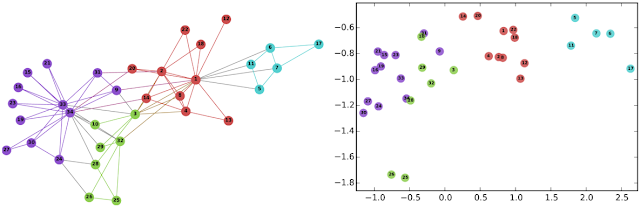
\includegraphics[width=0.8\linewidth]{fig/graph_embedding_intro.png}
\caption{对Karate network进行图嵌入的可视化,图源DeepWalk\cite{perozzi:deepwalk_kdd_2014}。}
\end{figure}

图嵌入方法主要可分为三类:基于\underline{矩阵分解}的方法、\underline{随机游走}(random walk)和\underline{图神经网络}(graph neural network, GNN)。
最早年使用的是基于矩阵分解的方法,但是计算量通常很大,只能处理图或结点特征维度较小的问题。
现在较多使用后两种方法,随机游走通常限制于转导(transductive)的设定,训练测试集属于同一个图;图神经网络则可以用于归纳(inductive)的设定,泛化能力强,可轻松适应未知的图/结点,因而GNN现在也成为应用和研究的热点。
% inductive个例到一般,可泛化
% transductive个例到个例,无法迁移到新输入
GNN已经在推荐系统\cite{zhu:aligraph_vldb_2019}、生物医学、程序综合、语义分割、逻辑推断等大量场景得到广泛应用。
% 阿里巴巴的电商平台现在部署了大量的GNN,包括GATNE[KDD'19]、Mixture GNN[KDD'19]、Hierarchical GNN[IJCAI'19]、Evolving GNN[IJCAI'19]等,在他们的推荐系统中起到至关重要的作用。不仅仅是阿里巴巴,其他互联网公司如Google、Twitter、Pinterest等,也面临着将这些GNN部署到\textbf{云端}高效执行的问题。
% 另外,计算机视觉领域最近大量采用GNN进行目标检测及语义分割,包括朱松纯老师的GPNN[ECCV'18]、梁小丹老师的SGR[NeurIPS'18]、代季峰老师的Relation Network[CVPR'18]等,这些模型在部署上\textbf{边缘}设备时必然也会产生模型过大、响应延迟高等问题。

但目前的GNN存在以下的问题:
\begin{itemize}
\item 从通用的图计算角度来讲,图具有不规则/非欧(non-Euclidean)结构和幂律分布(power-law)等特性,这与传统深度学习的稠密计算有着巨大差别,可扩展性差,没有办法处理大图。
然而现实世界中的社交网络、商品网络往往都是非常庞大的,要在这些图上采用GNN,算法复杂度一定是一个需要考虑的问题。
\item 从学习表示的角度来讲,现有的GNN更多捕获的是局部结构特征,而丧失了全局的相对位置信息。
这会导致GNN无法很好辨别同构子图结点,在一些预测任务上给出错误的结果。
一个简单的例子,一家三口在社交网络上呈现出来的都是三角形,但是GNN会认为所有这些三角形都是等同的(所有家庭没有区别),做图嵌入时会将这三个结点映射到同样的向量表示。
\end{itemize}

因此,本课题希望提出一种高效的图嵌入模型,在\textbf{保持局部和全局结构信息}的同时,具有\textbf{较高的可扩展性}。

\section{背景}
\subsection{记号}
考虑图$G(V,E)$,在其基础上添加顶点的类别,则形成标注图(labeled graph)$G_L=(V,E,X_{em},Y)$,其中$X_{em}\in\mathbb{R}^{|V|\times d}$为顶点嵌入,$Y\in\mathbb{R}^{|V|\times |\mathcal{C}|}$,$d$为特征维数,$Y$为标签集。
注意这种写法指$X$和$Y$均为矩阵,$X$一共有$|V|$行,每行对应一个顶点的特征向量,有$d$维;并且每个结点可能属于多个类别$\subset \mathcal{C}$。
图嵌入的目标是学习得到嵌入表示$X_{em}$,或者说映射$\Phi:V\mapsto X_{em}$,使得在低维的嵌入空间中,图结点有很好的\textbf{分布式连续表达},能够很好保持图的邻接结构,即结点向量间的距离能够衡量原图中的邻接关系强弱。
这里会涉及到不同的距离度量,不同的度量方式则会产生不同的图嵌入方法。

\subsection{随机游走}
随机游走顾名思义即从图上的一些结点$v$开始向它的邻居进行探索,采样出大量路径$\mathcal{N}_S(v)$后,对这些进行路径进行学习。

一个较通用的\textbf{优化目标}如下
\[\max_\Phi\sum_{v\in V}\log\mathrm{Pr}(\mathcal{N}_S(v)\mid \Phi(v))\]
即在生成的嵌入表示条件下,这种路径出现的概率尽可能大。

DeepWalk~\cite{perozzi:deepwalk_kdd_2014}最早使用随机游走来做图嵌入任务,每次随机选择一个起始点$v_i$,\textbf{随机选择邻居},做固定长度的随机游走,依据得到的$\mathcal{W}_{v_i}$,做skip-gram,梯度下降更新参数。

node2vec~\cite{grover:node2vec_kdd_2016}则不再采用DeepWalk每个结点完全随机的方式,而更加\textbf{有目的地利用BFS和DFS}进行采样。
可以看到这种方法对图的微观和宏观特性做了权衡,通过设置超参数$p$和$q$,能比较有效地学习到图的局部(BFS)和全局(DFS)特征。
\begin{figure}[H]
\centering
\begin{tabular}{cc}
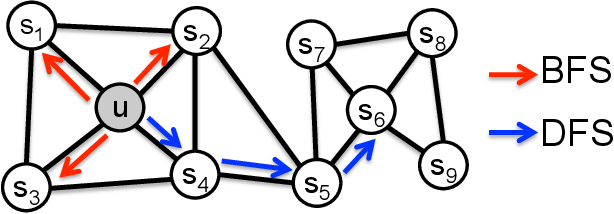
\includegraphics[width=0.6\linewidth]{fig/node2vec.png} &
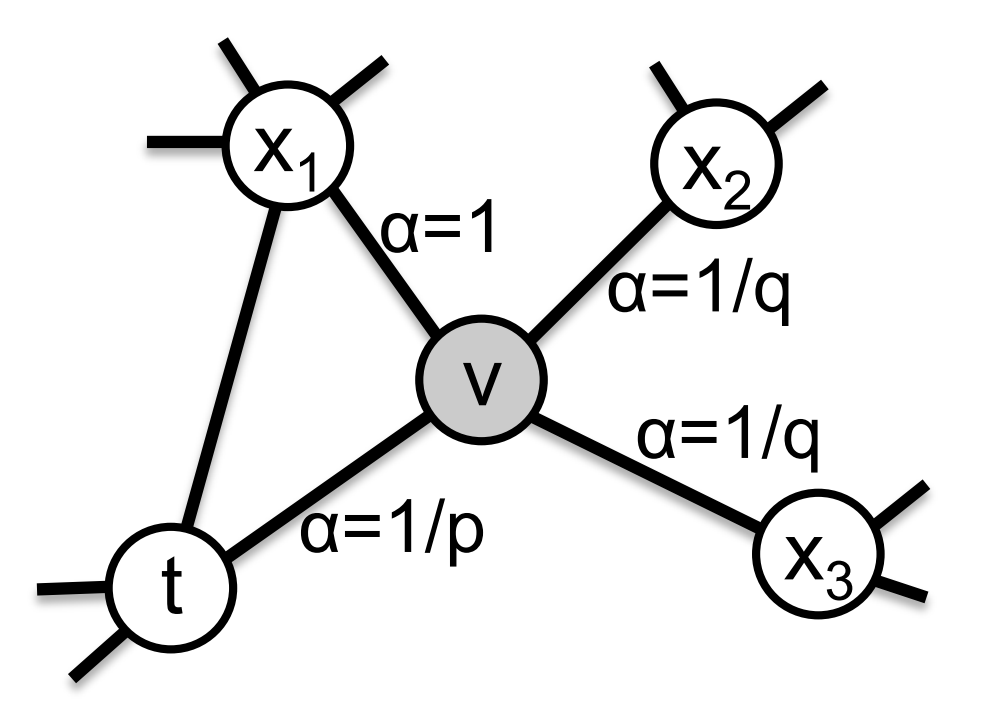
\includegraphics[width=0.3\linewidth]{fig/node2vec-transition.png}
\end{tabular}
\caption{node2vec~\cite{grover:node2vec_kdd_2016}状态转移}
\end{figure}

不同随机游走最大的差异在于其\textbf{邻居的选择}或在每个结点计算转移概率的方式\cite{yang:knightking_sosp_2019},这里可用统一的转移概率公式来表达%(注意这里并**未做归一化**)
\[P(e)=P_s(e)\cdot P_d(e,v,w)\cdot P_e(v,w)\]
这是十分直接的公式化,即某一条出边$e$的转移概率,等于静态成分、动态成分、扩展成分三者相乘。
详细地说,游走者$w$当前处于结点$v$,
\begin{itemize}
	\item 静态成分$P_s$只关乎当前的边$e$
	\item 动态成分$P_d$关乎这条边$e$以及游走者过来的路径/状态$w$%($w$含有$v$**之前**所有的状态)
	\item 扩展成分$P_e$则不与出边相关%(这里可能是为了解决其他一些未考虑到的情况,这一项的形式化方法存疑)
\end{itemize}

\subsection{图神经网络}
图神经网络的核心思想是从邻居\footnote{这里的邻居是泛化的邻居,不一定需要在图中真实相邻。}结点整合特征,通过不同神经网络架构进行拟合。
\begin{figure}[H]
\centering
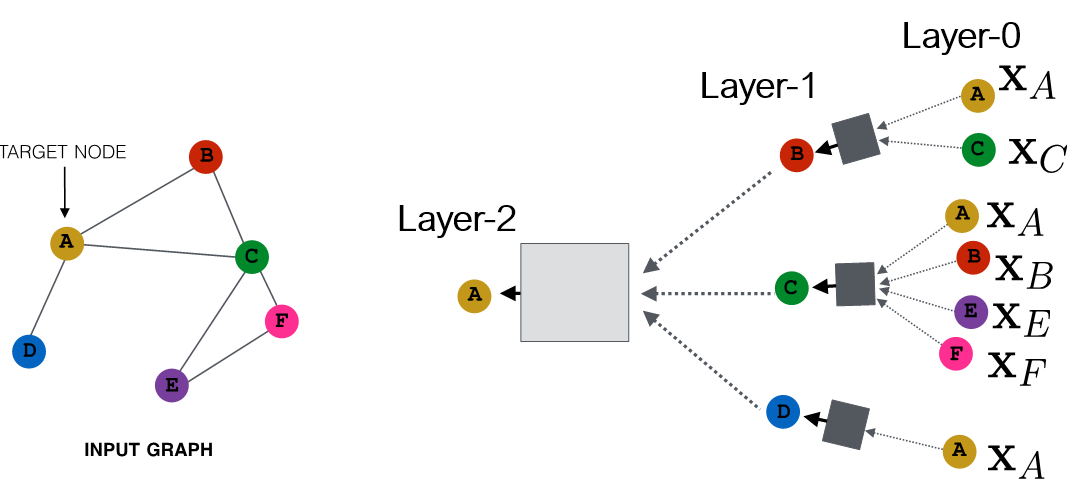
\includegraphics[width=0.8\linewidth]{fig/grl-layers.png}
\caption{图源Jure Leskovec, \href{http://snap.stanford.edu/proj/embeddings-www/}{Tutorial - Representation Learning on Networks (WWW'18)}}
\end{figure}

现有GNN的传播规则都可抽象为\cite{fey:pytorch_geo_2019}
\[\mathbf{v}_i^{(k+1)}=\gamma\left(\mathbf{v}_i^{(k)},\mathop{Agg}_{j\in\mathcal{N}_i}\phi(\mathbf{v}_i^{(k)},\mathbf{v}_j^{(k)},\mathbf{e}_{j,i}^{(k)})\right)\]
即包括\textbf{消息聚合}和\textbf{参数更新}两个步骤,其中$Agg$是一个可微、置换不变的函数(求和、求平均、求最值),$\gamma$和$\phi$则是可微函数(如MLP)。

最早提出的GCN~\cite{kipf:gcn_iclr_2017}很好地借鉴了传统CNN中卷积的思想,对网络层\textbf{共享参数},同时对自身特征进行聚合并做归一化,从而得到了更优的结果。
之后的GraphSAGE~\cite{hamilton:graphsage_neurips_2017}采用更加一般化的聚合函数,同时考虑合并(concat)自身特征而非相加的方式,进一步提升了GNN的性能。
其他各种GNN的变体,如GAT~\cite{velickovic:gat_iclr_2018}、GGS-NN~\cite{li:ggsnn_iclr_2016}等,在未经训练时其生成的图嵌入就已经达到随机游走的水准。

\section{动机}
我们可以看到,在去年的机器学习顶会上,已经有一些工作对一开始提出的两个问题进行了一定的研究。
这里最为显著的是Stanford的P-GNN~\cite{you:pgnn_icml_2019}和Cornell的GraphZoom~\cite{deng:graphzoom_iclr_2019}。

P-GNN提出了一种新型的GNN范式,整合位置信息,在结点预测任务上的提升是极其显著的,比现有GNN的准确率翻了超过一倍。
而GraphZoom则是近些年来第一次将GNN的适用范围推至billion级别的边数,可扩展性远超之前的GNN架构,速度提升最大达到40x加速比。
这两篇论文都说明在这波浪潮下,GNN可提升的空间依然很大。

\subsection{位置感知}
% http://snap.stanford.edu/pgnn/
GNN无法捕获全局相对的位置信息,导致对于相同的局部结构,其生成的结点嵌入相同,无法区分。
而这种结构等价性在分子结构、社交网络上却非常常见,因此有必要将位置信息也考虑在内。
\begin{figure}[H]
\centering
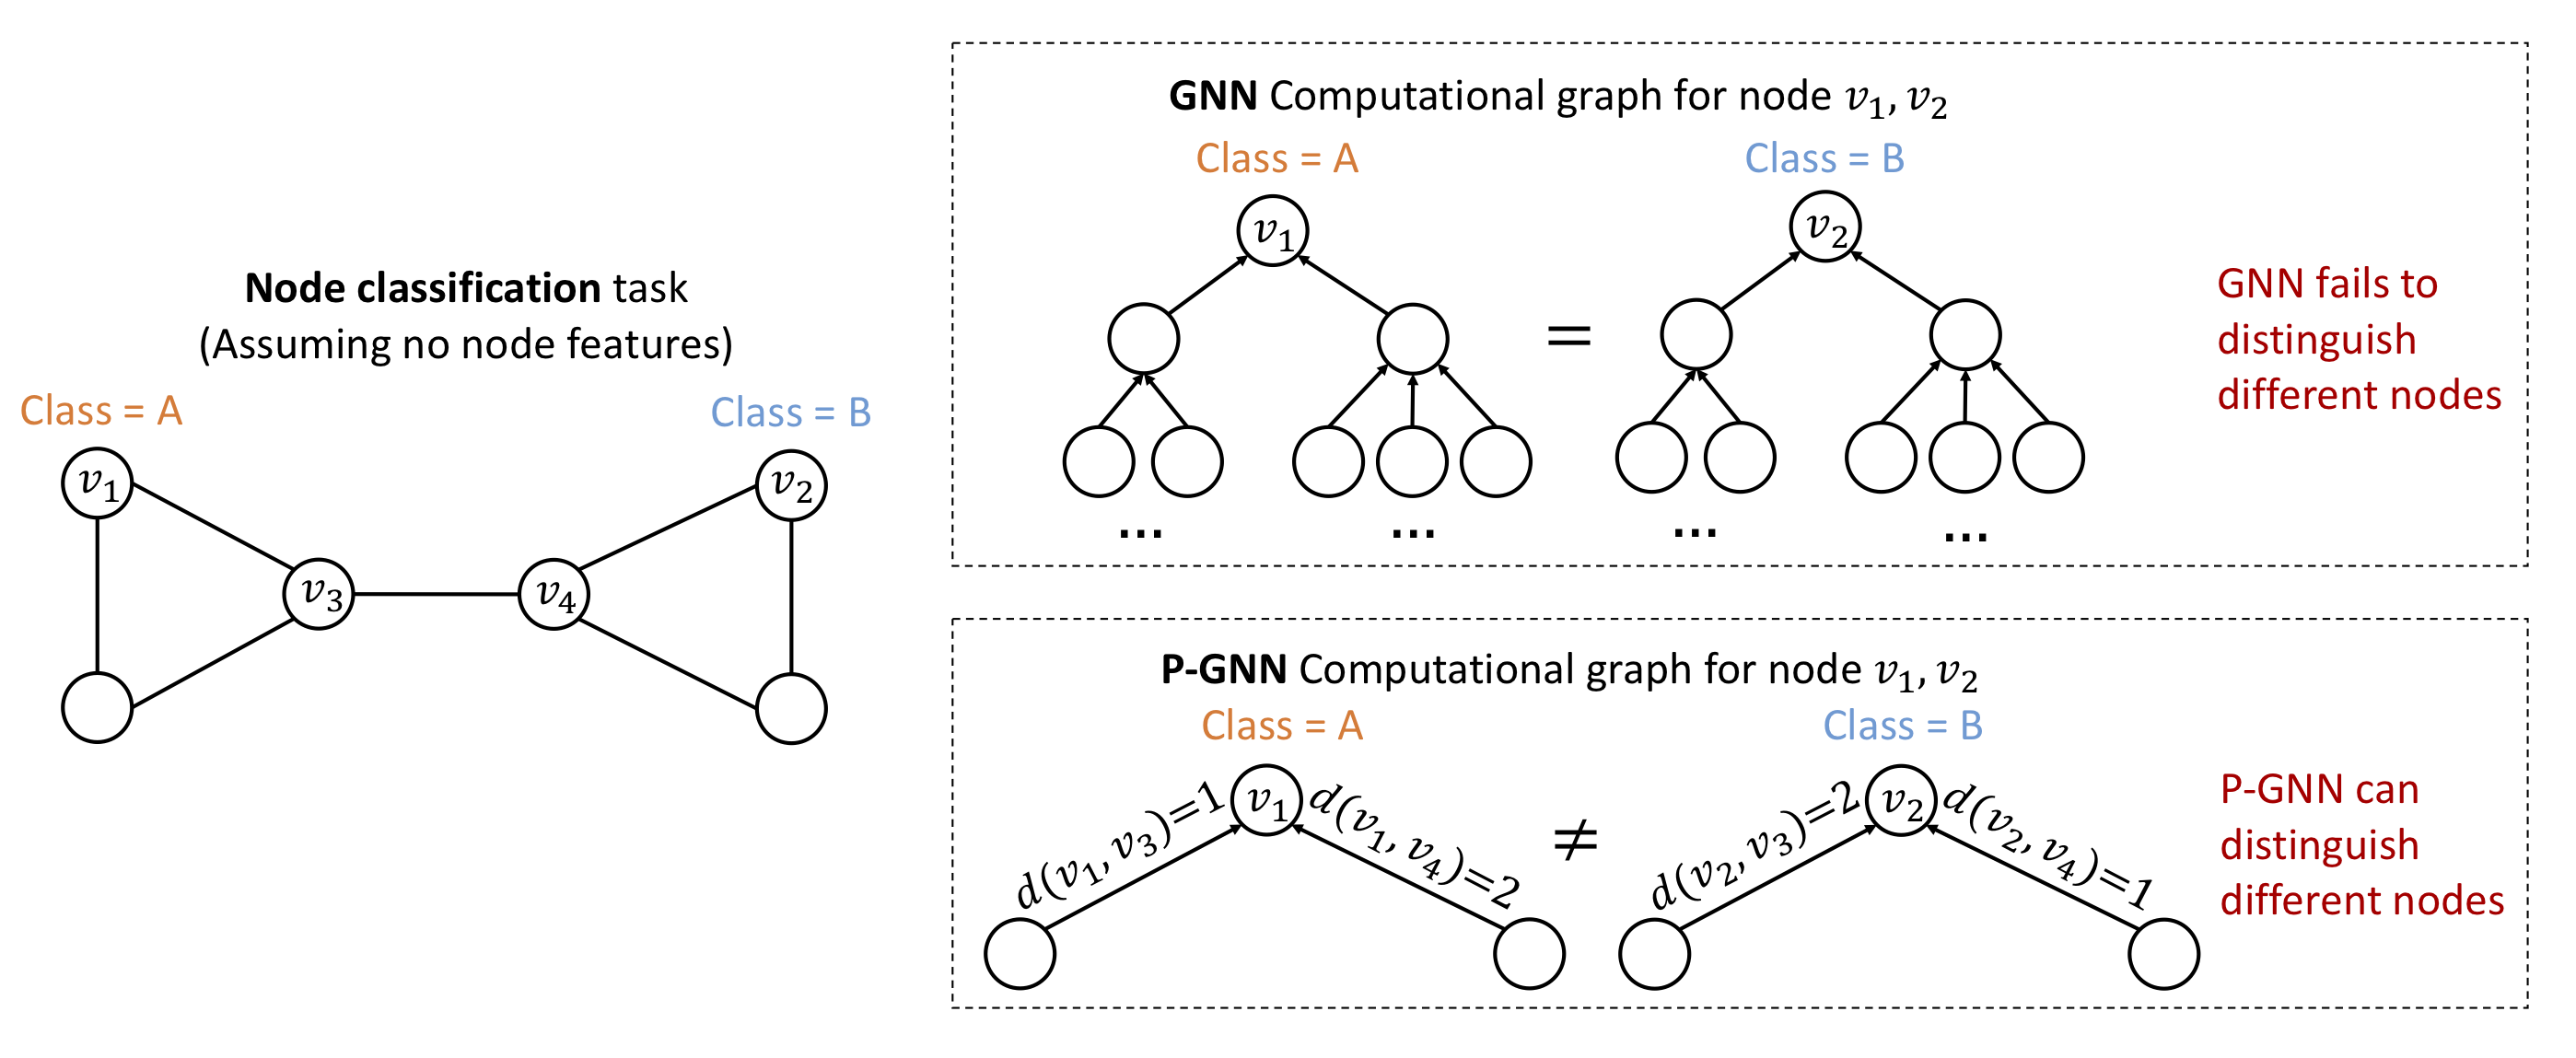
\includegraphics[width=0.8\linewidth]{fig/pgnn-example.png}
\caption{结构等价性}
\end{figure}
% 用独热码增量结点特征,让GNN更深

P-GNN每轮迭代中选取$k$个锚点(anchor)集(采样方式根据Bourgain定理),并将这些点作为其他所有点的邻居进行消息聚合。
而Bourgain定理说的是,给定$k=c\log^2n$个随机结点集$S_{i,j}\subset V,i=1,2,\ldots,\log n,j=1,2,\ldots,c\log n$,其中$S_{i,j}$以$1/2^i$的概率选取,以下列方式构造结点$v$的嵌入表示
\[f(v)=\left(\frac{d(v,S_{1,1})}{k},\frac{d(v,S_{1,2})}{k},\cdots,\frac{d(v,S_{\log n,c\log n})}{k}\right)\]
可以实现保位置变换,即在向量空间中相对位置信息不会被丢失。
\begin{figure}[H]
\centering
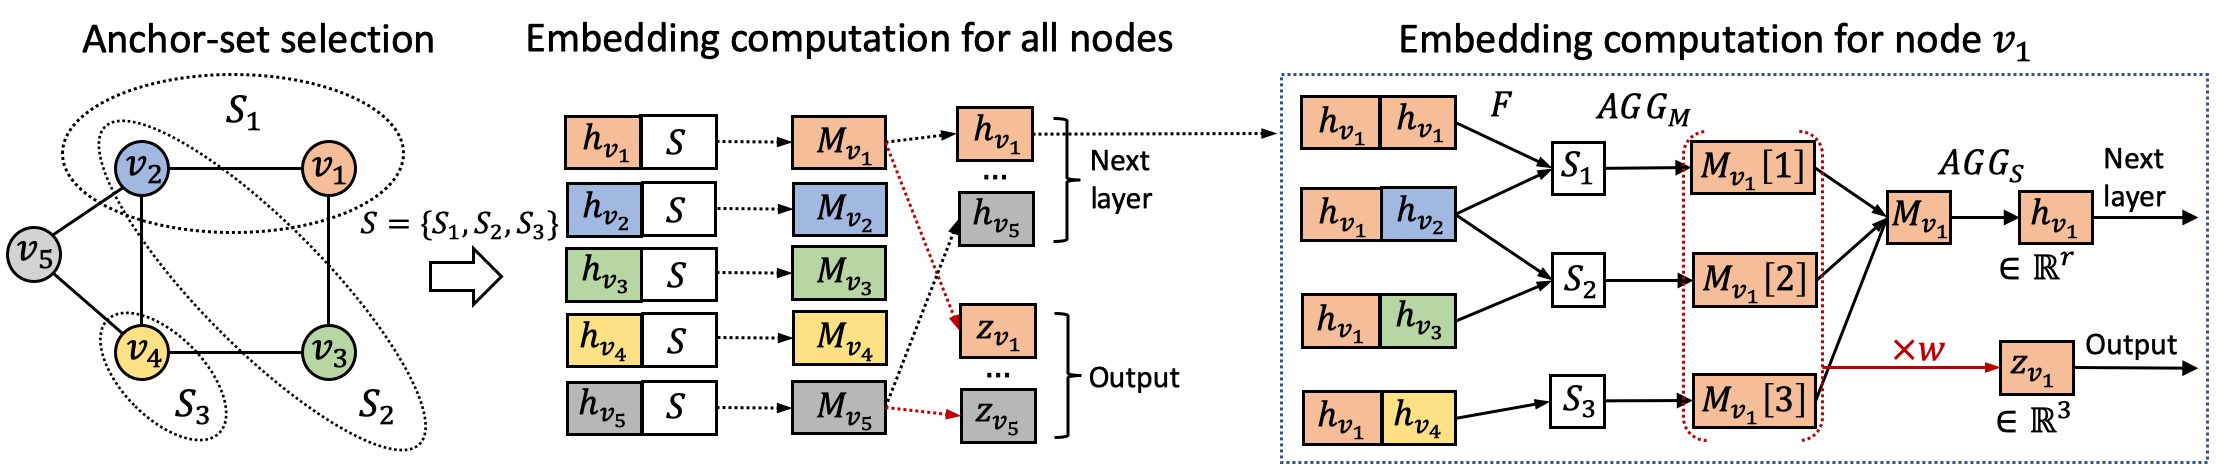
\includegraphics[width=0.8\linewidth]{fig/PGNN.png}
\caption{P-GNN生成图嵌入方式}
\end{figure}

这里的insight在于选定的锚点集有大有小,我们希望能够通过这些锚点来判断当前结点与其他结点的相对位置。
锚点集越大,碰到$v_i$的概率也就越高,有很高的采样效率,但是获得的信息量却很少;
而锚点集小,碰到$v_i$的概率也就小,那么信息量也就大,尽管采样效率低。

这其实是一个权衡,有点像图层面上的多尺度+空洞卷积,都是为了获得\textbf{更大的感受野},从而可以捕获局部和全局信息。
\begin{figure}[H]
\centering
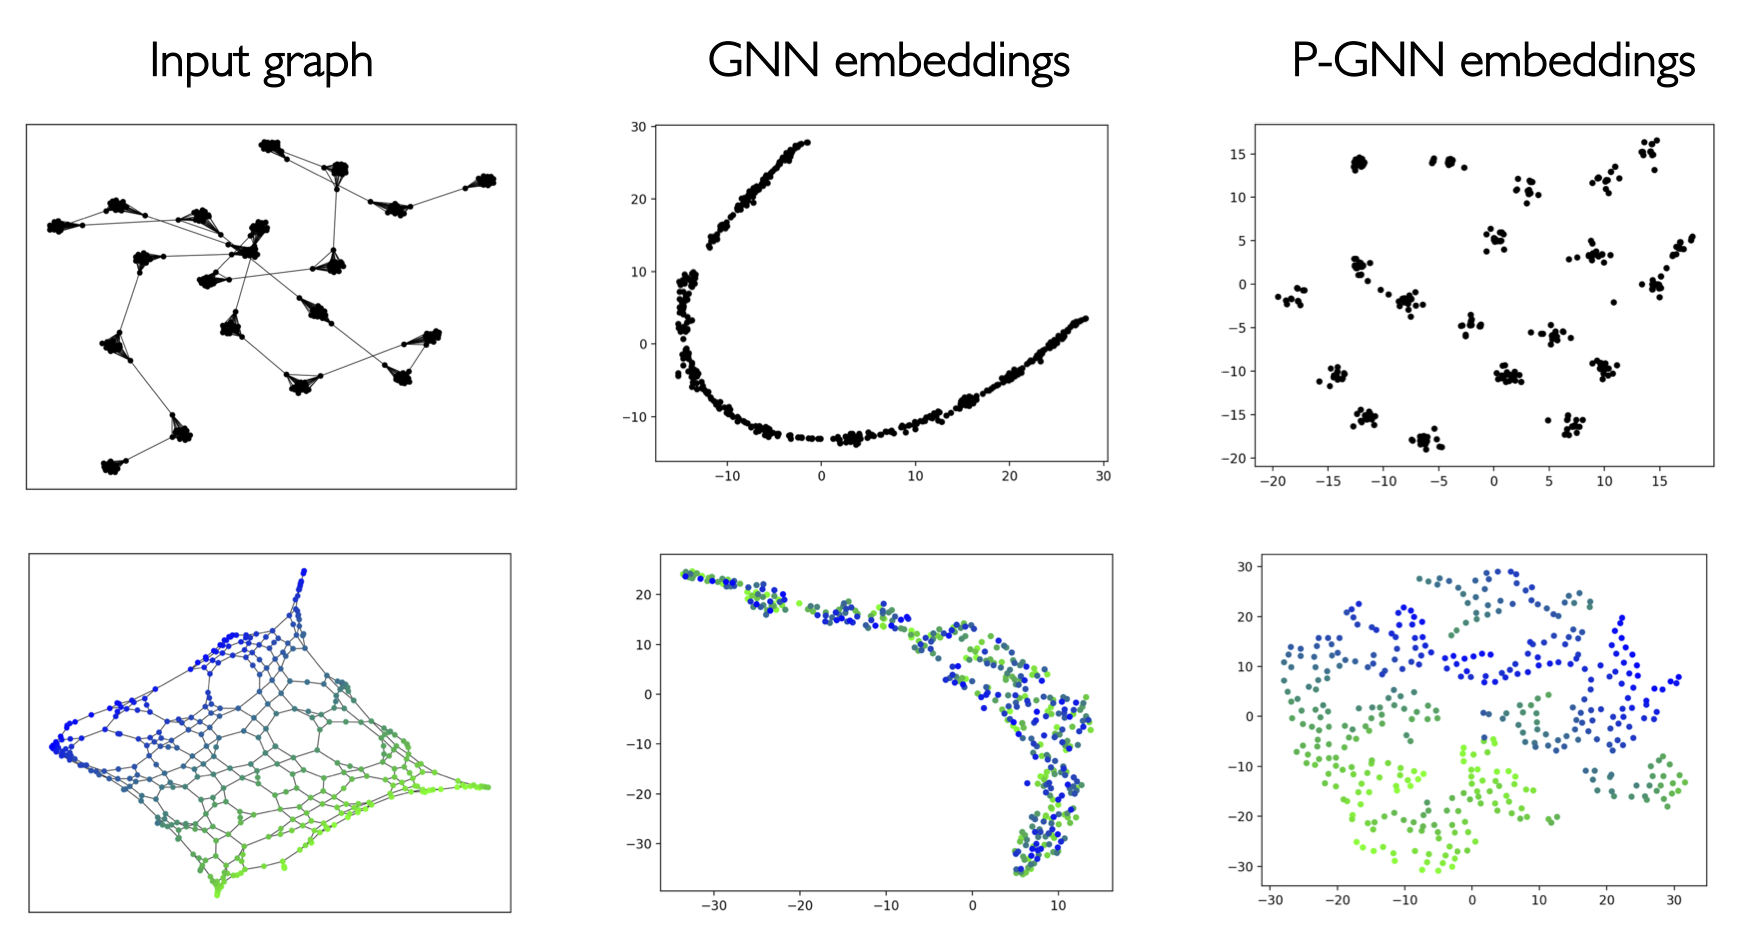
\includegraphics[width=0.8\linewidth]{fig/PGNN_results.png}
\caption{P-GNN结果可视化}
\end{figure}

% 位置感知:结点空间中的某种距离度量等同于于原始空间的距离,随机游走
% 结构感知:从当前节点往外扩的k跳可表为函数,GNN

从上面的叙述可知,P-GNN最大的开销在于锚点集的选取与通信,其消息通信复杂度是$O(mn\log^2 n)$,其中$m$为锚点集的平均结点数目,$n$为图的总结点数;
而现有的GNN通信代价一般都为$O(ne)$,所以P-GNN的开销还是非常大的。

为了降低这种开销,P-GNN在计算结点与锚点集的距离时采用$k$跳的截断估计法,事实上要计算SSSP依然开销很大。
\[d_{sp}^k(u,v)=\begin{cases}
d_{sp}(u,v) & d_{sp}(u,v)\leq q\\
\infty & \text{otherwise}
\end{cases}\]
% 结点标号敏感性
% 没有对特征进行处理,事实上特征中也会含有易于区别的位置信息。

\subsection{多级图嵌入框架}
大多数图嵌入方法都只提升准确率或者可扩展性当中的其中一个,而GraphZoom则尝试在提升可扩展性的同时,也提升预测的准确率。
其核心思想是融合结点特征后做降维再进行恢复。
\begin{enumerate}
	\item 图融合:邻接矩阵+结点特征\\
	Idea:基于属性相似度,对原始图做额外的边扩充(相当于提供了额外的信息)
	\begin{itemize}
		\item 基于L2范数利用kNN构建加权特征图(将结点属性矩阵转为图$A_{feat}$),权重为结点属性向量之间余弦相似度
		\item $A_{fusion}=A_{topo}+\beta A_{feat}$
	\end{itemize}
	\item 谱粗化(spectral coarsening):在谱图上做低通滤波,取前$k$大特征值进行重构
	\item 图嵌入:用现有图嵌入方法对粗化后的图做嵌入,主要是基于随机游走或GNN的方法
	\item 嵌入细化:拉普拉斯平滑后,映射回原图每一个结点
\end{enumerate}
\begin{figure}[H]
\centering
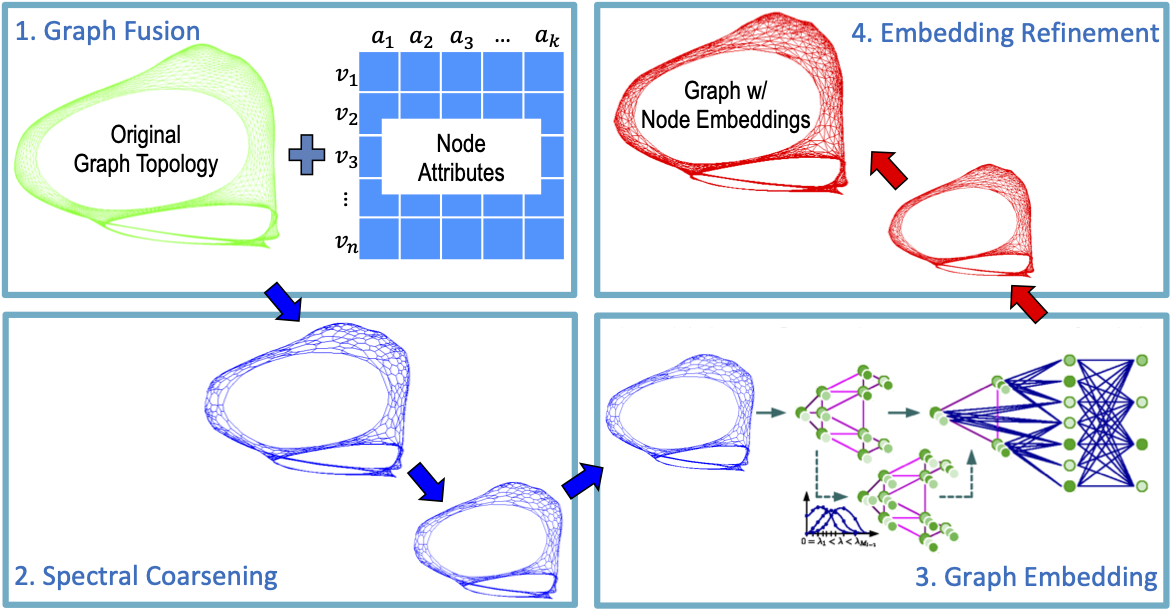
\includegraphics[width=0.8\linewidth]{fig/GraphZoom.png}
\caption{GraphZoom架构}
\end{figure}

这种方法很大程度上解决了可扩展性的问题,也证明了多尺度学习方法的有效性。
GraphZoom的核心问题在于变换过程中的信息保存度,降维后的图必然会丢失信息,那重要的那些位置信息是否丢失了,这是值得思考的。

\section{我们的方法}
既要维护位置信息,又要保持高可扩展性,意味着我们的方法不能太复杂。
维护位置信息需要兼顾局部和全局,保持高可扩展性又需要不能太关注于细节。
那么可以有以下两点研究思路:
\begin{itemize}
\item \textbf{高采样效率$\to$宽搜广搜结合}:P-GNN采用了一种非常随机的采样方式,尽管覆盖到了大锚点集也覆盖到小锚点集,但是效率太低,采用$k$截断算距离意味着大多数锚点集都是没有用的。
其实P-GNN的作者已经提到随机游走和GNN的问题,那么最直接的想法应该是将这两者结合。
可以参照node2vec~\cite{grover:node2vec_kdd_2016},采用BFS+DFS的方式来进行采样,而这两者的通信代价都只有$O(|E|)$。
\item \textbf{高可扩展性$\to$多尺度降维与恢复}:
降维不失为一种提速的方式,但是核心问题在于在降维后的图中的信息会丢失,因此怎么降以及怎么恢复是需要考虑的。
很多传统CNN的技术,可以尝试挪过来GNN这边使用,比如可以考虑类似UNet的架构,在恢复过程中复用前面的结果。
\end{itemize}

\bibliographystyle{IEEEtran}
\bibliography{graph}

\end{document}

% 2020.05.08 (individual): Mindmap based on the “research process and paper writing.pdf” file
% 2020.06.03 (team): intermediate report, partial information for introduction, related work, method, initial experimental results for at least one baseline method and your own initial idea.
% 2020.07.18 (team): final report together with source code.
% In addition, each team can make three appointments with me to discuss your project. I expect the first appointment is in early May for your initial ideas and related baseline methods, the second is in late May or early June for your initial results with your own idea and baseline methods, and the third is before late June for your well-developed idea and comprehensive result evaluation.